\atsptt
    \begin{frame}{\ft{Interacting with the Main Window}}
\section{Group 1: Interacting with the Main Window}

        \begin{annotatedFigure}{18pt}{0pt}
            {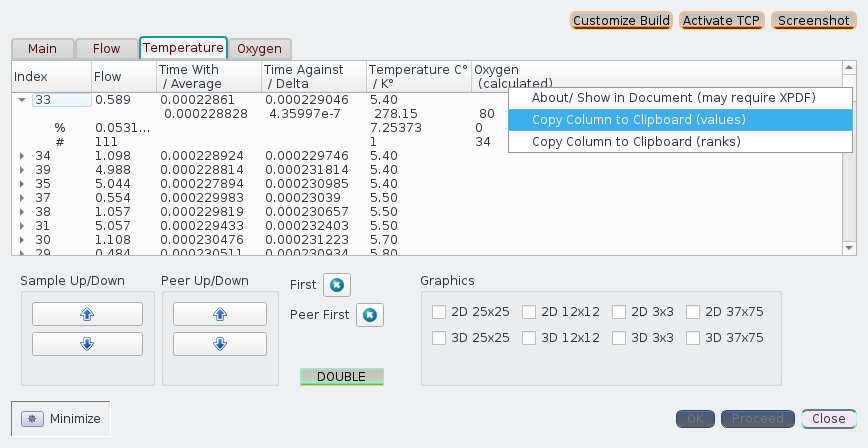
\includegraphics[scale=1.25]{texs/copy.png}}
            
  \node [text width=10cm,inner sep=14pt,align=justify,fill=logoCyan!20, draw=logoBlue, 
  draw opacity=0.5,line width=1mm, fill opacity=0.9]
   at (0.76,0.47){\annfont\textbf{Despite being implemented as a tree widget 
   instead of a two-dimensional spreadsheet, the primary 
   window for this Dataset Application has many speadsheet-like 
   features, such as copying columns of data 
   (\circled{1}) and sorting columns by switching 
   notebook tabs  (\circled{2}); each notebook page shows the data sorted 
   on a specific parameter.}};


      \annotatedFigureBox{0.93,0.67}{0.93,0.71}{1}{0.93,0.663}%
      \annotatedFigureBox{0.01,0.86}{0.34,0.935}{2}{0.17,0.85}% 
            
  \node [text width=11cm,inner sep=14pt,align=justify,fill=logoCyan!20, draw=logoBlue, 
  draw opacity=0.5,line width=1mm, fill opacity=0.9]
   at (0.59,0.2){\annfont\textbf{Two different sets of navigation buttons 
   enable the user to scroll through samples according to 
   the currently selected sort \mbox{parameter} (\circled{3}), 
   or according to the primary index (\circled{4}).}};

   \annotatedFigureBox{0.18,0.18}{0.33,0.41}{3}{0.33,0.41}%
   \annotatedFigureBox{0.02,0.18}{0.17,0.41}{4}{0.02,0.41}%    
      %      \annotatedFigureBox{0.222,0.284}{0.3743,0.4934}{B}{0.3743,0.4934}%tr
      %      \annotatedFigureBox{0.555,0.784}{0.6815,0.874}{C}{0.555,0.784}%bl
      %      \annotatedFigureBox{0.557,0.322}{0.8985,0.5269}{D}{0.8985,0.5269}%tr
  
        \end{annotatedFigure}

   %     \caption{Expanded Sample (A)}
    %    \label{fig:teaser}

    \end{frame}

